% \begin{figure*}[!hbp]
% \centering
% 
\includegraphics[width=1.0\textwidth]{2025_03/chris_durne.jpg}
% \centerline{\emph{Chris standing in front of the gold medal Bonsai display he curated at the Chelsea Flower Show.}}
% \end{figure*}
\headline{{\textbf{\Large\sffamily TWBC Workshops:}}\\
          {\textbf{\large\sffamily Bringing Bonsai Visions to Life}}}
\label{2025-03-workshop}
\noindent
Last Thursday's club meeting was all about bringing our bonsai design ideas to life---not with wire and shears, but with pencils and paper.
It was a wonderfully engaging evening that encouraged us all to step back from the practical aspects of bonsai care and instead focus on the creative vision for our trees.
The concept was simple yet deeply valuable: sketch out our bonsai's future, mapping its structure five and then ten years from now.
Whether we brought along a raw, unstyled sapling or a more developed tree in need of refinement, the exercise helped us clarify our long-term plans.
After all, shaping a bonsai is not just about responding to what's in front of us but envisioning what could be.

\medskip
\topic{Getting Started}
\noindent
\textit{Chris Durne} led the session, reminding everyone that artistic skill was not the focus.
This was not about producing a masterpiece fit for an exhibition but about translating our thoughts onto paper.
The tools were basic---A4 or A3 paper, pencils (preferably soft, like HB or 2B), an eraser for those who liked a clean slate, and coloured crayons to indicate foliage, flowers, or even seasonal changes.
We began with the simplest form: the \textit{``stick tree.''} As amusing as it might sound, drawing a basic trunk and primary branches in this stripped-back way was a great way to start.
It allowed us to focus on structure before getting lost in the details.
Once our stick trees were in place, we started adding depth, imagining how they would develop over time.
This is where personal creativity came in.
Some of us kept things quite minimal, sketching light, wispy outlines of potential branch development.
Others got more technical, considering specific wiring techniques or how a planned deadwood feature might evolve.

\medskip
\topic{Five Years Forward}
\noindent
The next step was to think about the five\--year mark.
We asked ourselves key questions:

\begin{itemize}
    \item How much will the trunk have thickened?
    
    \item Which branches will we encourage, or remove?
    
    \item How will the canopy begin to take shape?
    
    \item What sort of seasonal changes will the tree exhibit?
\end{itemize}

Sketching this stage was particularly fun, as it allowed us to play with ideas.
Some members experimented with different possibilities, drawing multiple versions of their tree to explore alternative styling directions.
Chris encouraged everyone to think in terms of layering---starting with the main structural elements and then lightly indicating secondary branches and foliage pads.
Using coloured crayons, we highlighted leaf masses and floral areas, making it easier to visualise how our designs would mature.

\columnbreak

% \medskip
\topic{A Decade of Growth}
\noindent
Looking a decade ahead took even more imagination.
We had to consider refinement---how the tree would shift from development to a mature, styled bonsai.
This was where we truly saw the benefits of long\--term thinking: a branch planned for year five might not be needed by year ten.
Others spotted chances for bolder features like exposed roots, shari, or jin.
It was a fascinating exercise, reminding us that bonsai is a patient art and the best results come from thoughtful progression.

\medskip
\topic{Sharing and Learning}
\noindent
One of the best parts of the night was seeing the variety of approaches taken.
Some trees had a natural, flowing design, while others took on more dramatic, angular forms.
The diversity of ideas was inspiring.
More importantly, the atmosphere was relaxed and encouraging.
As Chris had promised, there was no judgment---only curiosity and shared enthusiasm.
Those who were less confident with drawing were supported by others who had more experience.
There was plenty of discussion, with members offering friendly suggestions and insights based on their own trees and styling experiences.

\medskip
\topic{Takeaways from the Session}
\noindent
By night's end, everyone left not just with sketches but with a clearer bonsai direction.
Some even noticed mistakes in their current styling---things they might have missed without putting pencil to paper.
This exercise was a great reminder of the importance of stepping back and visualising our trees' future.
When working on a bonsai, it's easy to get caught up in the moment, making small tweaks without a clear plan.
Drawing forces us to slow down and see the bigger picture.

\medskip
\topic{Looking Ahead}
\noindent
Workshops like this one highlight why our club meetings are so valuable.
They're not just about learning techniques but about developing a deeper connection with our trees and each other.
If you missed this session, don't worry---we'll have plenty more opportunities to explore bonsai design and styling in the months ahead.
In the meantime, why not try a sketching session at home?
Grab a pencil, pick a tree, and start imagining its future.
You might be surprised by what you discover!

\begin{window}[%
    2,l,%
    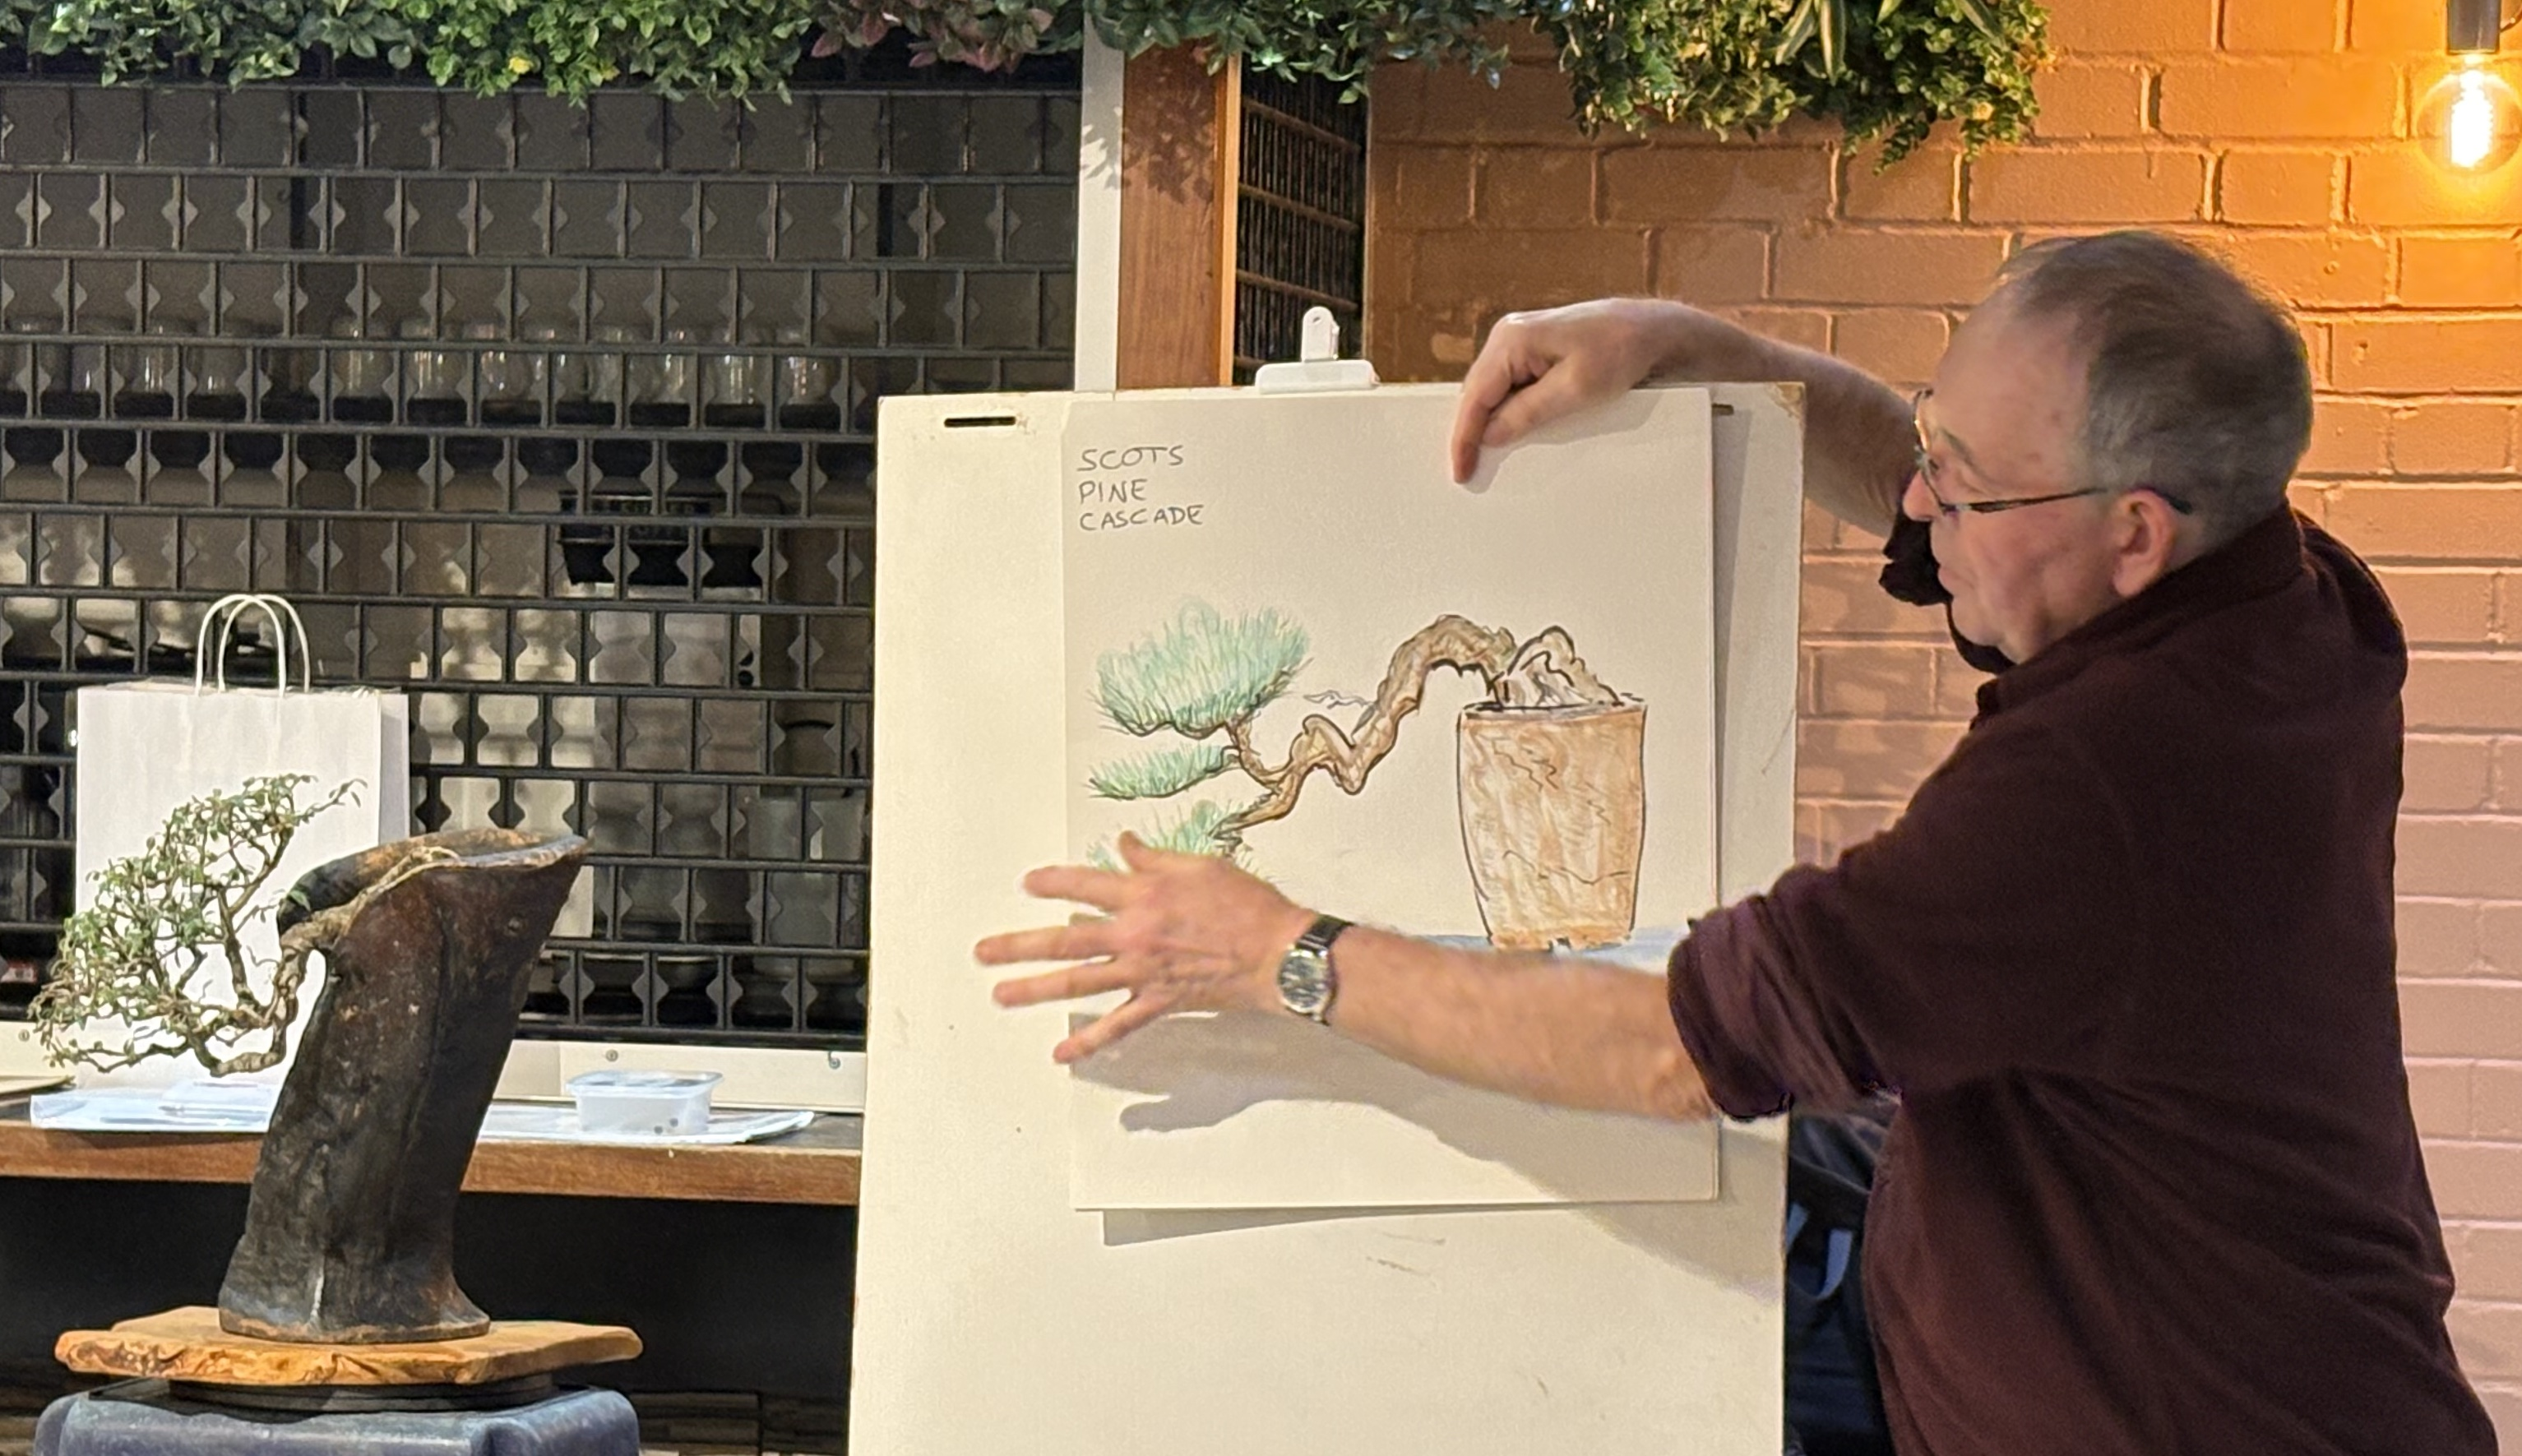
\includegraphics[width=1.0\columnwidth]{2025_03/res/workshop_chris_durne},%
    \centerline{\emph{From tree to vision---Chris breaks down workshop's key ideas.}}%
]
\end{window}
\closearticle
\columnbreak
